\section{Component Model}



\subsection{Frontend}
%TODO Peter Schmucki

\subsection{Backend}
Zur Organisation der Backend Sourcen orientieren wir uns an der Onion-Architecture.
Die Umsetzung wird aufgrund der geringen Projektgrösse jedoch nicht in unabhängigen Modulen realisiert, sondern über die Package Struktur angedeutet.
Bei der Implementation wird dennoch konsequent darauf geachtet, die einzelnen Layer so zu halten das diese als eigenständige Module extrahiert werden können.

Die erwarteten Layer sind:
\begin{itemize}
    \item Core
    \subitem Model der Dokumente
    \subitem Business Logik zur Konsistenz garantie
    \subitem Command Engine
    \item Service
    \subitem Schnittstelle zwischen Persistenz und API zum Core
    \item Persistence
    \subitem Anbindung an das Datenbanksystem
    \item API
    \subitem Controller für eingehende Dokument Updates
    \subitem Controller für die Reaktive-Streams zu den aktiven Clients.
\end{itemize}

\begin{figure}
    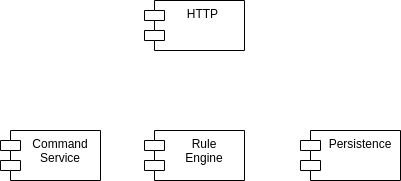
\includegraphics[width=\textwidth,height=\textheight,keepaspectratio]{simple-componentModel}
    \caption{Simple Backend Component Model}
\end{figure}
